\documentclass[11pt, a4paper]{article}
\input{preamble.tex}
\switchlang{ru}
\begin{document}

\title{1982 "--- A2D Joystick 2001}
\date{}
\maketitle
\selectlanguage{russian}

A2D Joystick 2001 (рис. \ref{fig:A2DJoystick2001Pic}) "--- это аналоговый джойстик второго поколения от компании A2D для компьютеров Apple II. Он был представлен на рынке в 1982 году и оказался своего рода <<работой над ошибками>> на фоне первой модели, вышедшей двумя годами ранее и имевшей некоторые изъяны в эргономике. Джойстик продавался одновременно с похожим на него манипулятором типа <<колесо>>, A2D Paddles, модель 2002 \cite{a2d_paddles}.

\begin{figure}[h]
   \centering
    
\includegraphics[width=\textwidth]{1982_a2d_joystick_2001/pic_30.jpg}
    \caption{A2D Joystick 2001}
    \label{fig:A2DJoystick2001Pic}
\end{figure}

\section*{Внешний вид}

Внешний вид устройства претерпел большие изменения относительно первой модели, копировавшей вид пультов дистанционного управления радиоуправляемых моделей самолетов. Корпус джойстика A2D 2001 выполнен из бежевого пластика, имеет компактную форму в виде параллелепипеда с закругленными углами. Как и у первой модели, на торце по-прежнему расположены две кнопки, однако теперь они снабжены крупными колпачками с вогнутой поверхностью, которые гораздо удобнее нажимать пальцами (рис. \ref{fig:A2DJoystick2001TopAndBottom}). На противоположной от кнопок стороне находится табличка с логотипом компании-производителя. Низ корпуса совершенно плоский, лишен каких-либо элементов, в том числе ножек. На верхней стороне присутствует только стик и триммеры для механической корректировки положения потенциометров, позволяющей выставить нулевое напряжение для каждой из осей. Рукоятка джойстика достаточно стандартная: начиная со второй половины 1970-х годов, её можно встретить в ряде профессиональных контроллеров курсора (например, в джойстике Tektronix 4952 для графических компьютерных терминалов или джойстике DEC H3060, разработанном для семейства мини-компьютеров PDP-11).

\begin{figure}[h]
    \centering
    
\includegraphics[scale=0.65]{1982_a2d_joystick_2001/top_30.jpg}
    
\includegraphics[scale=0.65]{1982_a2d_joystick_2001/bottom_30.jpg}
    \caption{A2D Joystick 2001, вид сверху и снизу}
    \label{fig:A2DJoystick2001TopAndBottom}
\end{figure}

\section*{Размеры}

Общие габариты устройства уменьшились по сравнению с первой моделью A2D; корпус стал заметно короче, но немного шире. В результате корпус модели 2001 (рис. \ref{fig:A2DJoystick2001Size}) очень компактен по меркам настольных джойстиков, но «немного великоват для того, чтобы его было удобно держать в руке среднестатистического пользователя». Корпус похожих размера и формы (и кстати, колпачки кнопок) получила модель A2D Paddles 2002: из-за этого она оказалась заметно больше, чем большинство игровых типа «колесо», представленных на рынке \cite{a2d_paddles}.

\begin{figure}[h]
    \centering
    
\includegraphics[scale=0.4]{1982_a2d_joystick_2001/size_30.jpg}
    \caption{A2D Joystick 2001 на размерном коврике с шагом сетки 1~см}
    \label{fig:A2DJoystick2001Size}
\end{figure}

\section*{Эргономика}

Отсутствие логотипа на верхней стороне и «квадратные» пропорции устройства вызвали большие разногласия по поводу правильного способа его держать. В частности, вариант с нажатием кнопок большим пальцем руки, держащей устройство, предложенный в обзорах \cite{a2d_paddles} и \cite{info_3}, был категорически раскритикован в открытом письме президента A2D Company \cite{a2d_answer}, сообщающем, что «попытка активировать кнопки большим пальцем... будет достаточно неудобной», так как устройство «предназначено для удержания в руке и активации кнопок ее [остальными] пальцами», и что «кнопки расположены на передней части корпуса, а не на задней», вопреки утверждению в \cite{a2d_paddles} (положение «передней части» относительно пользователя при этом не уточняется). Вероятное положение джойстика в руках при таком использовании иллюстрирует рисунок \ref{fig:A2DJoystick2001TwoHands}. Интуитивным такое положение рук назвать трудно, но по крайней мере оно работоспособно.

\begin{figure}[h]
    \centering
    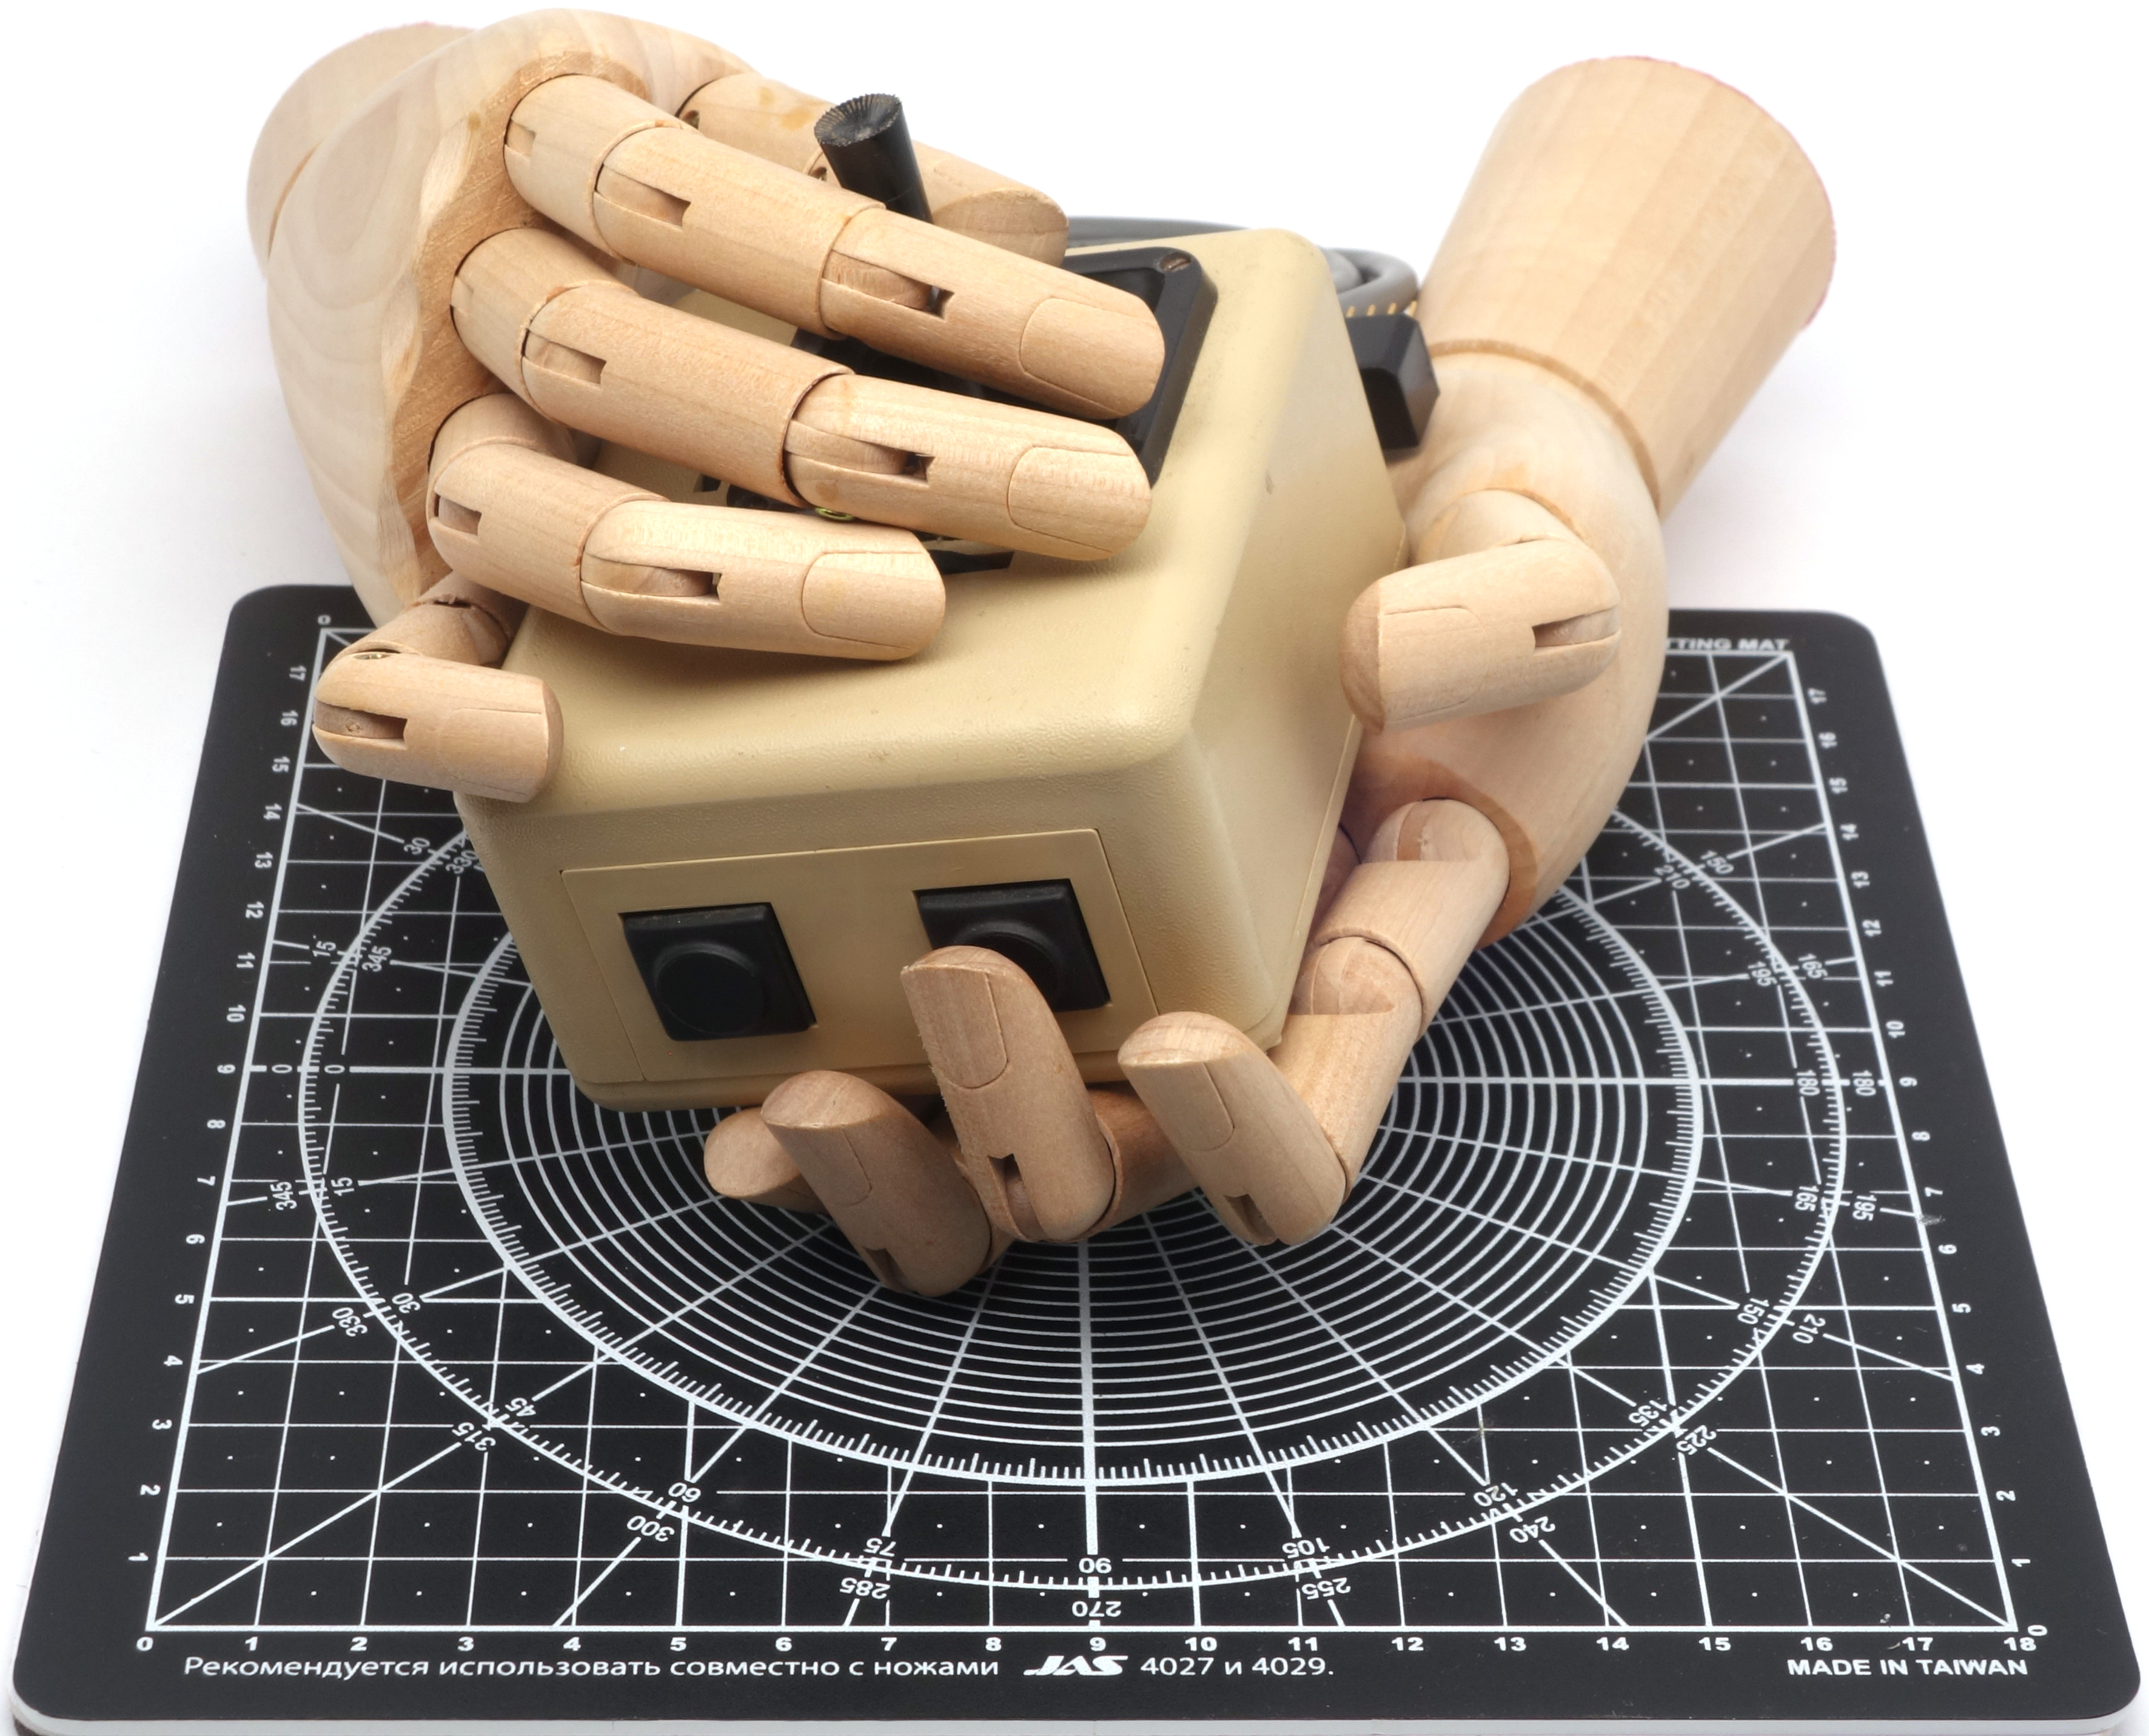
\includegraphics[scale=0.45]{1982_a2d_joystick_2001/hand2_30.jpg}
    \caption{A2D Joystick 2001 с моделью руки человека, удерживание в руке}
    \label{fig:A2DJoystick2001TwoHands}
\end{figure}

Однако, как можно заметить по рисунку \ref{fig:A2DJoystick2001Hand}, настольное использование джойстика оказывается по меньшей мере не менее удобным в случае, когда пальцы одной руки одновременно придерживают корпус и нажимают на кнопки, а пальцы другой управляют стиком.

\begin{figure}[h]
    \centering
    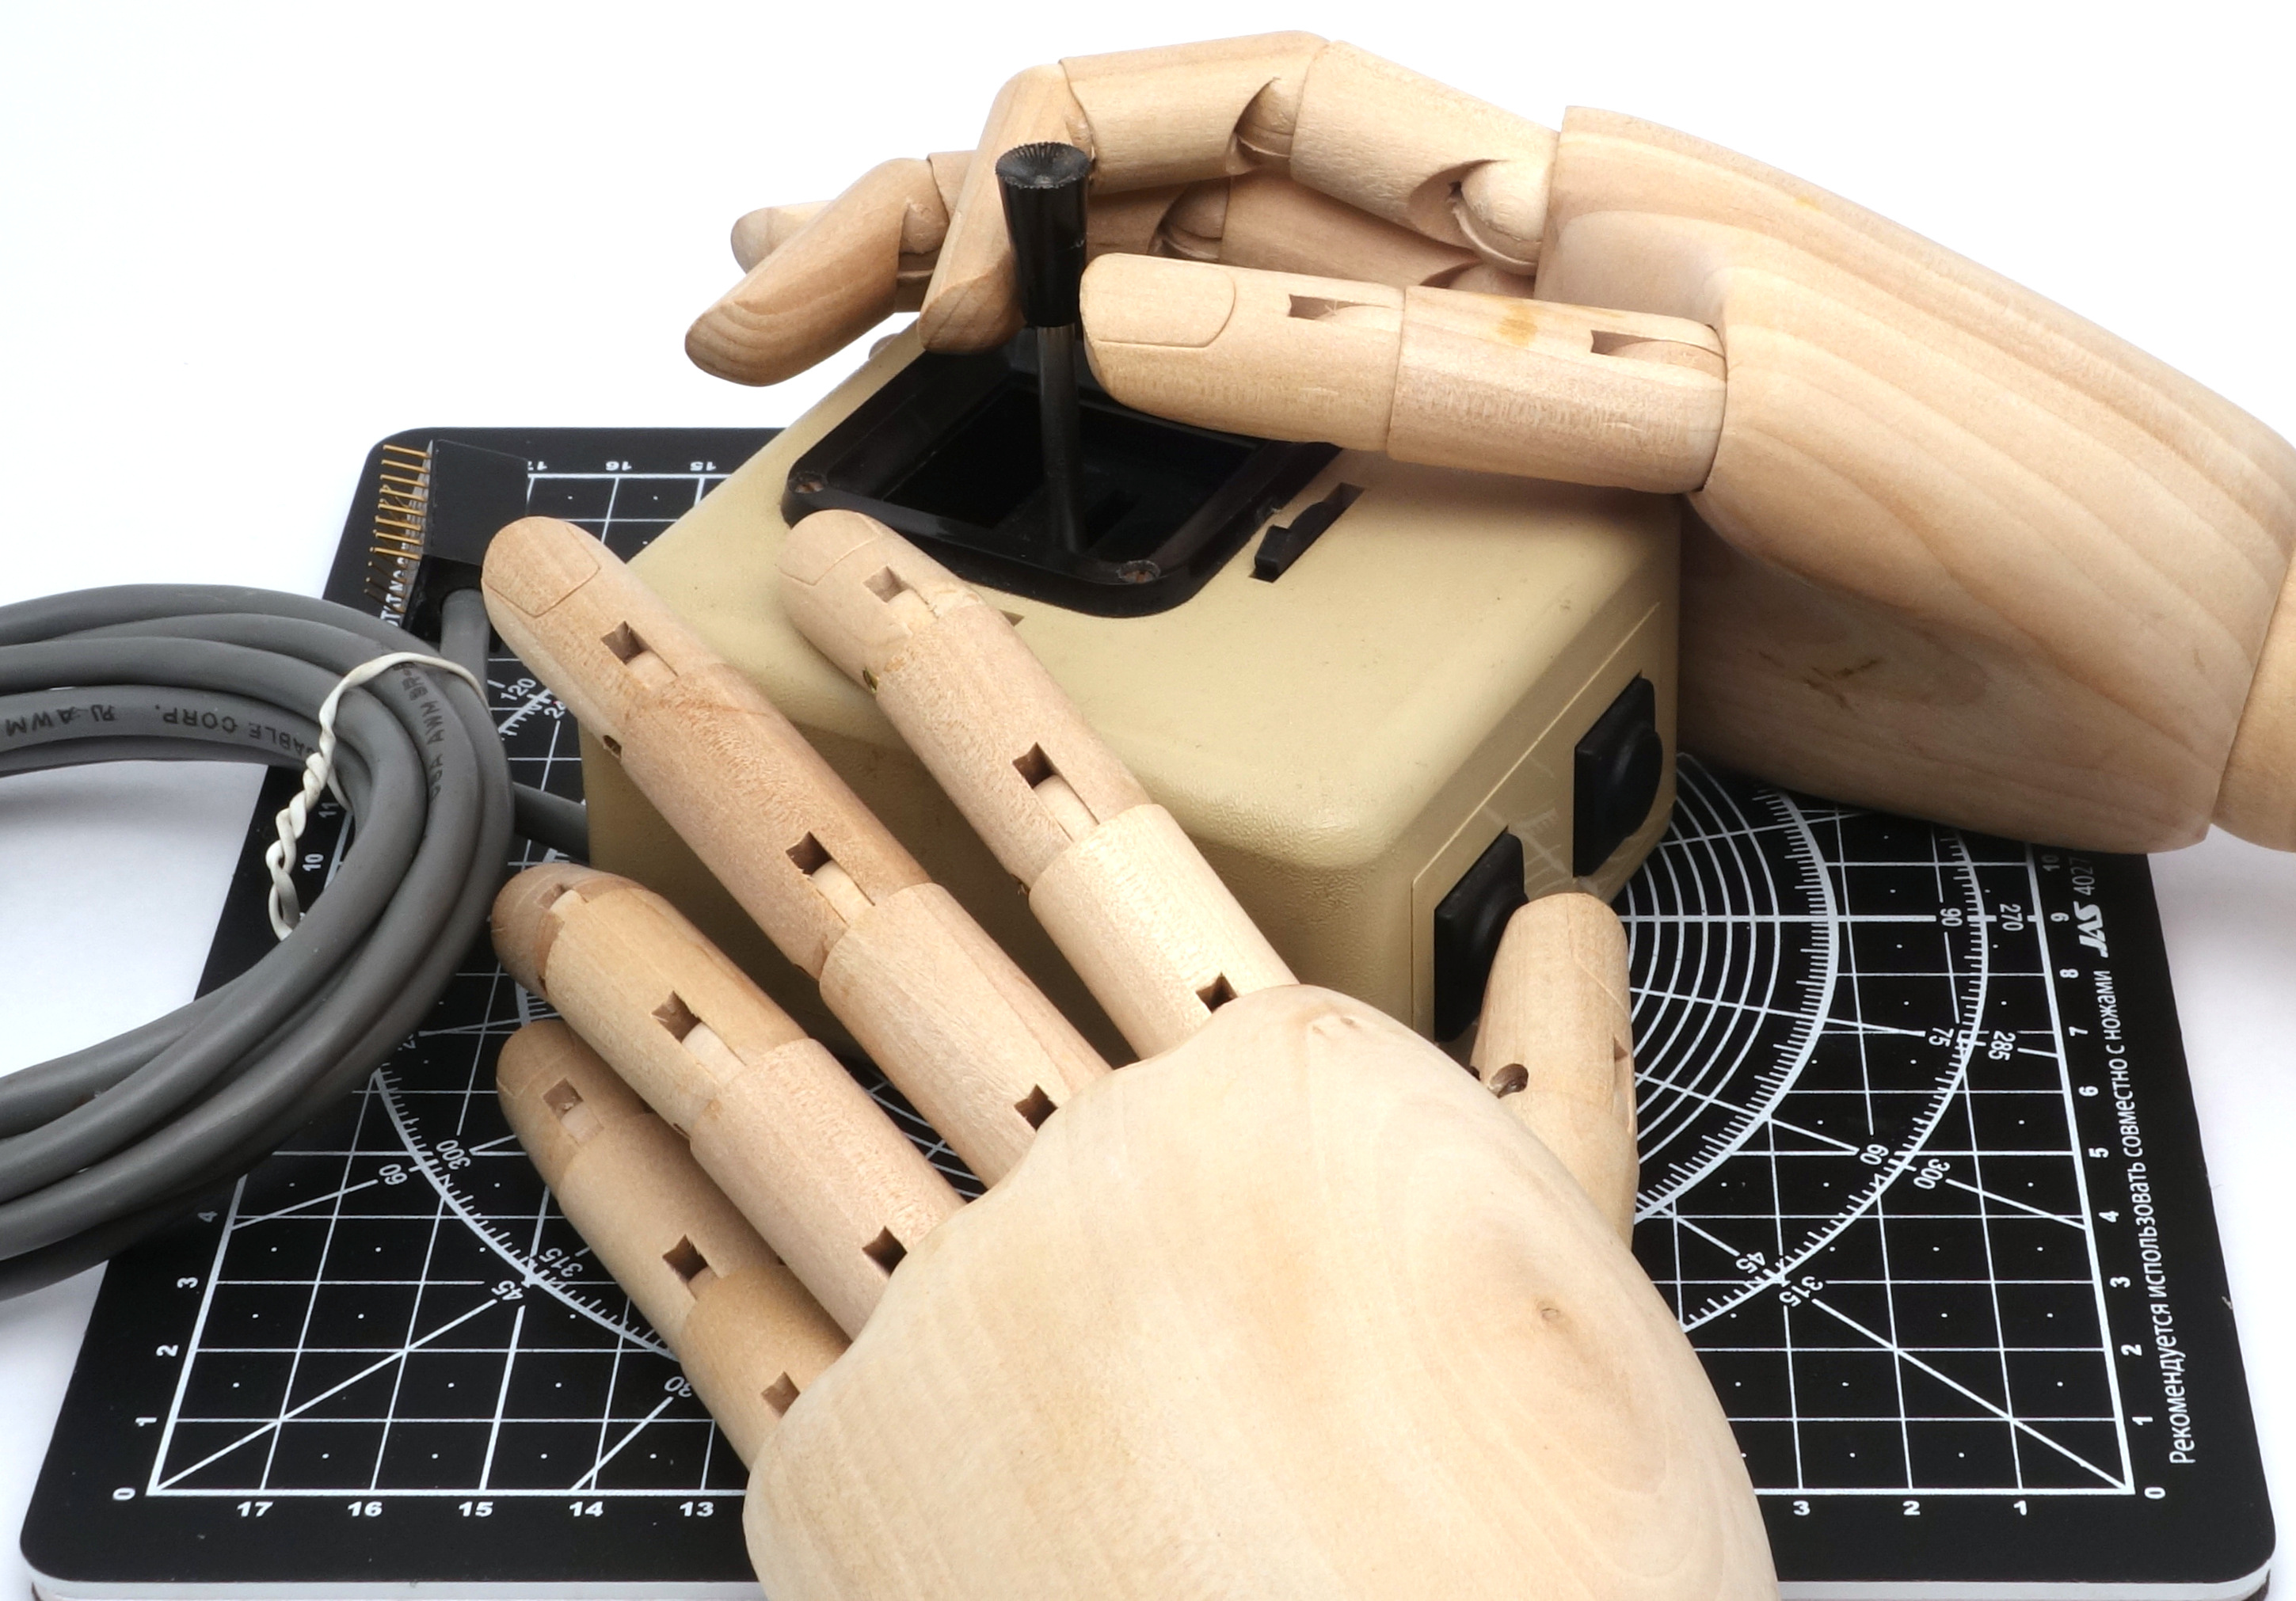
\includegraphics[scale=0.54]{1982_a2d_joystick_2001/hand3_30.jpg}
    \caption{A2D Joystick 2001 с моделью руки человека, настольное использование}
    \label{fig:A2DJoystick2001Hand}
\end{figure}

Рукоятка от традиционных джойстиков управления курсором в устройстве, разработанном в первую очередь для игр, несколько дезориентировало целевую аудиторию, но, как отмечается в \cite{info_3}, при использовании устройства с удерживанием стика пальцами это не создавало существенных проблем в играх. Там же отмечено большое улучшение кнопок по сравнению с первой моделью: они большие, с вогнутыми колпачками, «имеют очень короткий ход и обеспечивают отличную тактильную и звуковую обратную связь».

Как и в первой модели, узел джойстика, включая весь электромеханический блок, был намеренно заимствован из пультов дистанционного управления радиоуправляемых моделей. Эта связь намеренно подчеркивалась упоминанием «прецизионного джойстика с открытым карданным подвесом» \cite{joustickAD}, «разработанного для соревнований по аэробатике на радиоуправляемых моделях» \cite{joystick81}. Авторы обзоров отмечают его «очень плавное и точное действие» \cite{a2d_paddles}.

\section*{Внутреннее устройство}

В разобранном виде джойстик показан на рис. \ref{fig:A2DJoystick2001Inside}). Конструкция узла джойстика является достаточно стандартной, основанной на аналоговых потенциометрах, преобразующих отклонение рукоятки в изменение электрического сопротивления. Как и пультов управления радиомоделями, стики A2D Joystick действительно размещены на активно рекламировавшихся производителем металлических карданных подвесах (gimbal). Также можно отметить использование оттрассированной вручную коммутационной печатной платы (вместо проводного монтажа, использованного в предыдущей модели).

Устройство по-прежнему не имеет винтов для отключения режима самоцентрирования джойстика (они были добавлены в более поздней модели). В одном из обзоров тем пользователям, кому это нужно, предлагалось исправить ситуацию вручную, разобрав джойстик и вынув пружины \cite{a2d_paddles}.

\begin{figure}[h]
    \centering
    
\includegraphics[width=\textwidth]{1982_a2d_joystick_2001/inside_30.jpg}
    \caption{A2D Joystick 2001 в разобранном виде}
    \label{fig:A2DJoystick2001Inside}
\end{figure}

\begin{thebibliography}{9}

\bibitem {a2d_paddles} J. Mazur. Hardtalk // Softalk, Vol.2, No 8, April 1982 -- p.58. \url{https://archive.org/details/softalkv2n08apr1982/page/57/mode/2up}

\bibitem {info_3} Ahl D.H. Joysticks, Paddles, and Game Port Extenders. Potentiometer Joysticks. A2D Joystick (2001) // Creative Computing, Vol.8, No 8, August 1982 -- p. 79. \url{https://archive.org/details/creativecomputing-1982-08/page/n79/mode/2up} % 82

\bibitem {a2d_answer} Porter H. Buttons Up, Thumbs Down // Softalk, Vol.2, No 10, June 1982. -- P. 24. \url{https://archive.org/details/softalkv2n10jun1982/page/24/mode/2up}

\bibitem {joustickAD} A2D Joystick 2001 (advertising) // Creative Computing, Vol.8, No 12, December 1982 -- p. 238 \url{https://archive.org/details/CreativeComputing1982-12/page/n231/mode/2up}

\bibitem{joystick81} Van Diver G., Love R. Apple II/III software directory. Vital Information, Inc., 1981. p. PR-21 \url{https://archive.org/details/vanlovesappleiii00gera/page/470/mode/1up?q=a2d+joystick}

\end{thebibliography}
\end{document}
